% Generated by pipeline/paper/scripts/make_result_figures.py. Do not edit by hand.
% R2p tie-break. Count of tblout rows inside the consistency predicate. n=578.
% Shared figure style. Input once; a second input is a no-op.
\ifdefined\actsplotsready
\else
  \def\actsplotsready{1}
  \colorlet{actsteal}{teal!72!black}
  \colorlet{actstealfaint}{teal!16}
  \colorlet{actsorange}{orange!88!black}
  \colorlet{actsink}{black!80}
  \colorlet{actsghost}{black!45}
  \colorlet{actsfail}{red!62!black}
  \colorlet{actsrule}{black!50}
  \usetikzlibrary{intersections}
  \usepgfplotslibrary{fillbetween,groupplots}
  \pgfplotsset{
    acts/.style={
      font=\scriptsize\sffamily,
      tick label style={font=\scriptsize\sffamily},
      label style={font=\scriptsize\sffamily},
      legend style={
        font=\scriptsize\sffamily,
        draw=none,
        fill=none,
        cells={anchor=west},
        inner sep=1pt,
        column sep=6pt
      },
      legend cell align=left,
      scale only axis,
      clip=false,
      axis line style={actsrule},
      tick style={actsrule},
      tick align=outside,
      axis lines=left,
      xmajorgrids=true,
      major grid style={black!7},
      ymajorgrids=false,
      every node/.append style={font=\scriptsize\sffamily, inner sep=1.5pt},
      every axis plot/.append style={line join=round, line cap=round},
    },
  }
  \tikzset{
    actlab/.style={
      font=\scriptsize\sffamily,
      fill=white,
      fill opacity=0.92,
      text opacity=1,
      inner sep=1.35pt,
      outer sep=0.5pt,
    },
  }
\fi

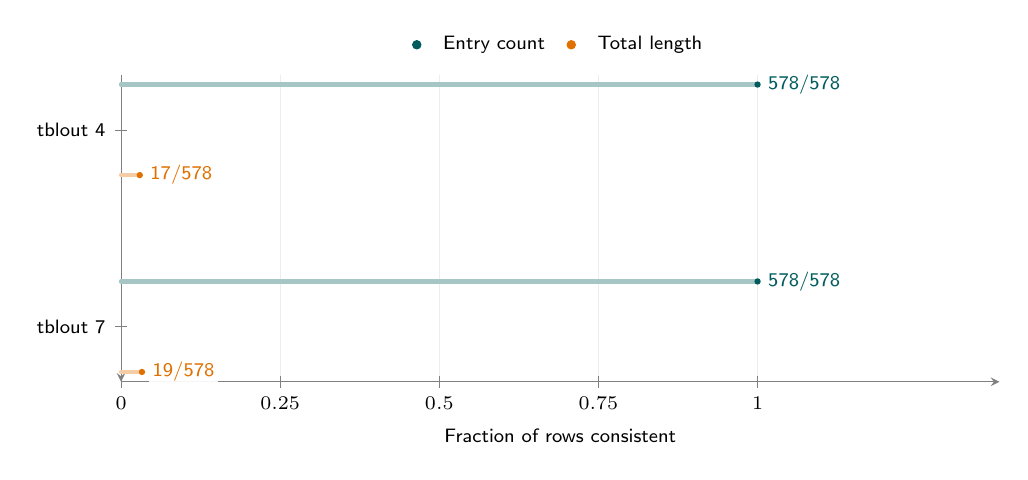
\begin{tikzpicture}
\begin{axis}[
  acts,
  width=0.92\columnwidth,
  height=3.90cm,
  xmin=0, xmax=1.38,
  xtick={0,0.25,0.5,0.75,1},
  xlabel={Fraction of rows consistent},
  ytick={0,...,1},
  yticklabels={{tblout 4},{tblout 7}},
  y dir=reverse,
  enlarge y limits=0.28,
  legend style={at={(0.5,1.04)}, anchor=south, legend columns=2},
]
\addplot[draw=none, forget plot] coordinates {(0,0) (1,1)};
\addlegendimage{only marks, mark=*, mark size=1.5pt, fill=actsteal, draw=actsteal}
\addlegendimage{only marks, mark=*, mark size=1.5pt, fill=actsorange, draw=actsorange}
\addlegendentry{Entry count}
\addlegendentry{Total length}
% source: reference_fitter_t1.json r2p tie_break entry_count
\draw[actsteal!35, line width=1.6pt, line cap=round] (axis cs:0,-0.2300) -- (axis cs:1,-0.2300);
\fill[actsteal] (axis cs:1,-0.2300) circle[radius=1.15pt];
\draw[actsteal!35, line width=1.6pt, line cap=round] (axis cs:0,0.7700) -- (axis cs:1,0.7700);
\fill[actsteal] (axis cs:1,0.7700) circle[radius=1.15pt];
% source: reference_fitter_t1.json r2p tie_break total_entry_length
\draw[actsorange!35, line width=1.6pt, line cap=round] (axis cs:0,0.2300) -- (axis cs:0.029411765,0.2300);
\fill[actsorange] (axis cs:0.029411765,0.2300) circle[radius=1.15pt];
\draw[actsorange!35, line width=1.6pt, line cap=round] (axis cs:0,1.2300) -- (axis cs:0.032871972,1.2300);
\fill[actsorange] (axis cs:0.032871972,1.2300) circle[radius=1.15pt];
\node[actlab, anchor=west, text=actsorange, xshift=2pt] at (axis cs:0.029411765,0.2300) {17/578};
\node[actlab, anchor=west, text=actsteal, xshift=2pt] at (axis cs:1,-0.2300) {578/578};
\node[actlab, anchor=west, text=actsorange, xshift=2pt] at (axis cs:0.032871972,1.2300) {19/578};
\node[actlab, anchor=west, text=actsteal, xshift=2pt] at (axis cs:1,0.7700) {578/578};
\end{axis}
\end{tikzpicture}
